\documentclass{article}

% Language setting
% Replace `english' with e.g. `spanish' to change the document language
\usepackage[spanish]{babel}

% Set page size and margins
% Replace `letterpaper' with `a4paper' for UK/EU standard size
\usepackage[a4paper,top=2cm,bottom=2cm,left=3cm,right=3cm,marginparwidth=2cm]{geometry}

% Useful packages
\usepackage{amsmath}
\usepackage{graphicx}
\usepackage[colorlinks=true, allcolors=black]{hyperref}
\usepackage{fancybox}
\usepackage{listings}
\usepackage{subcaption}
%\lstset{
%    language=Matlab,
%    extendedchars=true
%}

\title{Comportamiento del protocolo Aloha Ranurado}
\author{Álvaro Hernández Riquelme}
%\date{}

\begin{document}
\maketitle

\tableofcontents
\newpage

%\begin{abstract}
%Your abstract.
%\end{abstract}


\section{Introducción al trabajo}

Para este trabajo, se estudiará el comportamiento de un protocolo de Aloha Ranurado usando un sistema SDL, donde se completará la edición, simulación y validación total del protocolo. Tras esto, se hará un estudio de éste.

\quad

\textbf{SDL}, también conocido como Simulation and Description Language, es el lenguaje de especificación formal creado por la ITU para definir y representar sistemas y protocolos. Se usará la herramienta \textbf{Telelogic Tau}, para representar nuestra especificación de \textbf{Aloha Ranurado}. Tendremos una base sin terminar del protocolo en el aula virtual, la cual modificaremos y completaremos, finalmente haremos una simulación y validación. 

\quad

\textbf{Aloha} es un protocolo de acceso al medio aleatorio, donde varios nodos pueden compartir información con una probabilidad de colisión, ya que se envía la información sin comprobar si el canal está libre. Quiere decir que si en el tiempo de envío, existe otro nodo transmitiendo, se producirá ésta colisión. Para mejorar las prestaciones, se define \textbf{ALOHA ranurado}, donde se dividen las transmisiones de mensajes en slots del tamaño de éste mensaje y los nodos solo pueden transmitir al inicio de los slots. De este modo, se reduce el periodo de colisión.

\subsection{Nuestro Entorno}

Como se ha dicho previamente, usaremos Telelogic Tau para la simulación del protocolo. Al abrirlo, si cargamos la base del trabajo proporcionada en el aula virtual, podremos empezar a trabajar sobre ésta.

\quad

\begin{figure}[h]
    \centering
    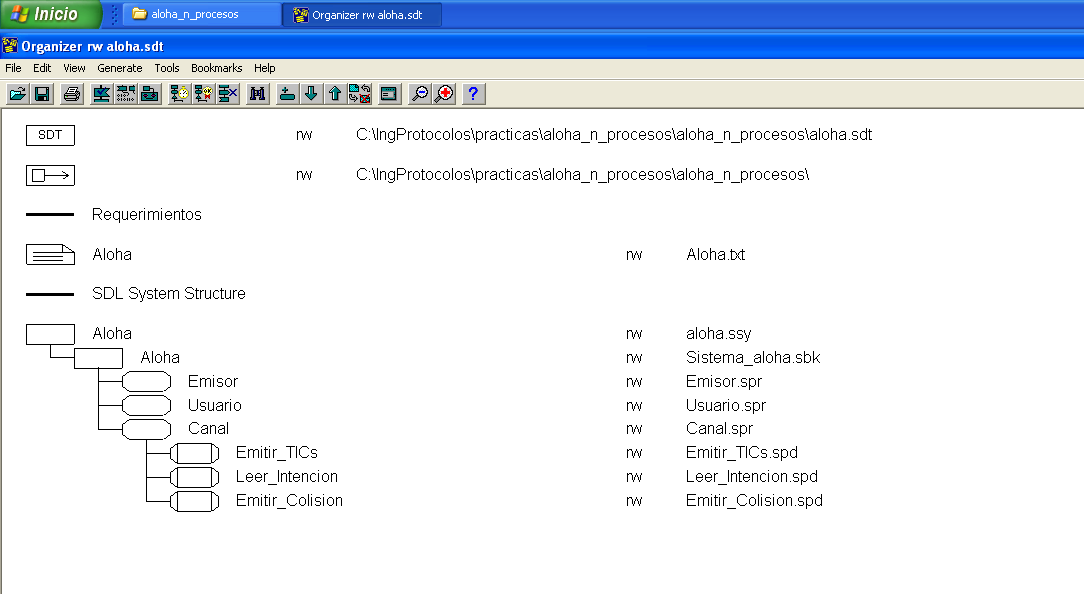
\includegraphics[width=1\linewidth]{src/Organizer-tltau.png}
    \caption{\label{fig:tltau} Inicio de Telelogic Tau con el proyecto de ALOHA Ranurado.}
\end{figure}

\newpage

\section{Edición}

Como se nos ha comentado en clase, antes de ir a la simulación y validación, tendremos que emepzar con la edición, ya que la base proporcionada no está completa. Teniendo en cuenta la captura anterior, y usando el programa para ver qué hay hecho, vemos que los estados \textbf{Emisor, Usuario, y Canal} están sin terminar, por lo que empezaremos diseñando estos estados.
Es importante reconocer qué significa cada símbolo:

\begin{figure}[h]
    \centering
    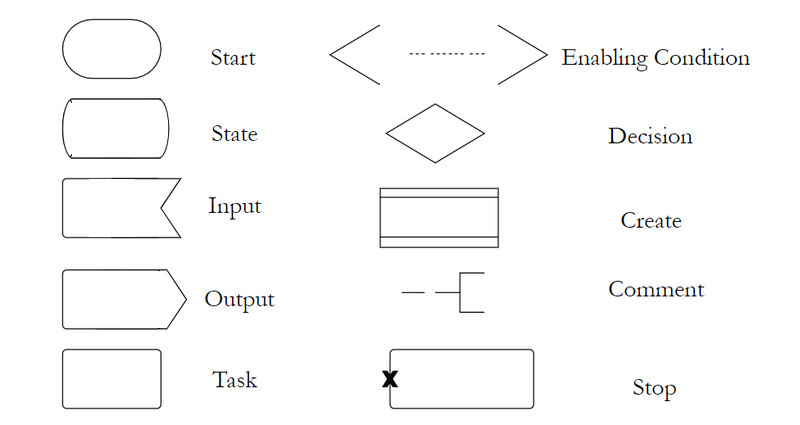
\includegraphics[width=0.7\linewidth]{src/sdl-symbols.jpg}
    \caption{\label{fig:sdlsymbols} Significado de los símbolos en SDL.}
\end{figure}

\quad

\subsection{Emisor}

\subsection{Usuario}

\subsection{canal}


\end{document}